\section{The Metropolis-Hastings Algorithm}

\textit{Metropolis-Hastings algorithm} is one of the most used \textit{Markov Chain Monte Carlo}(MCMC) algorithm.
The \textit{Metropolis algorithm} was first introduced by Nicholas Metropolis in 1953 in his paper entitled \textit{"Equation of State Calculations by Fast Computing Machines"}, with Arianna W. Rosenbluth, Marshall Rosenbluth, Augusta H. Teller and Edward Teller.
Arianna Rosenbluth wrote the first full implementation of Metropolis Algorithm for  \textit{Mathematical Analyzer Numerical Integrator and Automatic Computer Model I}(MANIAC 1) which was an early computer built under the direction of Nicholas Metropolis at the Los Alamos Scientific Laboratory.

\begin{figure}[H]
	\centering
	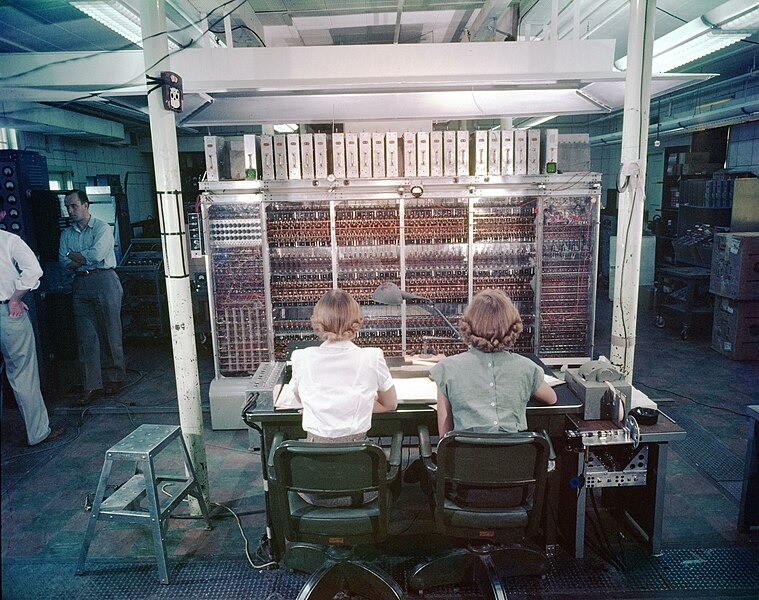
\includegraphics[width=0.4\textwidth]{Operators_in_front_of_the_MANIAC.jpg}
	\caption{MANIAC 1 one of the earliest computer.}
	\label{MANIAC}
\end{figure}

For many years this algorithm was simply known as \textit{Metropolis Algorithm}, later in 1970 W.K. Hastings introduce more general version of this algorithm in his paper \textit{"Monte Carlo Sampling Methods Using Markov Chains and Their Applications"}. This generalized Metropolis algorithm is known as \textit{Metropolis-Hastings algorithm}(MH algorithm).

Suppose we want to simulate a random variables or sequence of random variable with probability mass function
\begin{equation}
	\pi(\theta) = \frac{f(\theta)}{K}
\end{equation}
where $ K $ is normalizing constant which is unknown or difficult to compute.

One way to simulate $ \pi(\theta) $ is to constant a Markov Chain that is easy to simulate and whose limiting distribution is $ \pi(\theta) $.
The \textit{Metropolis-Hastings algorithm} do exactly this. MH algorithm constant a time-reversible Markov Chain with desired limiting probabilities.

\subsection{Algorithm for Metropolis-Hastings}
\begin{enumerate}
	\item Start with any \textbf{initial state}  $ \theta_0 $ satisfying $ f(\theta) > 0 $.
	\item Using a \textbf{current state}  $ \theta $, sample \textbf{candidate state} $ \theta' $ for some \textbf{jumping distribution} $ q(\theta, \theta') = q(\theta'|\theta) $, which is the probability of jumping to $ \theta' $ provided the current state in $ \theta $.
	\item Given the candidate state $ \theta' $ calculate the \textbf{acceptance probability} $ \alpha(\theta,\theta') $ by,
	      \[
		      \alpha(\theta,\theta') =\min\left( \frac{\pi(\theta')q(\theta', \theta)}{\pi(\theta)q(\theta, \theta')}, 1\right) = \min\left( \frac{f(\theta')q(\theta', \theta)}{f(\theta)q(\theta, \theta')} , 1\right)
	      \]
	\item  Accept the candidate point with probability $ \alpha $.

\end{enumerate}
We can summarize the Metropolis-Hastings Algorithm as first computing,
\[
	\alpha(\theta_{t},\theta_{t+1}) = \min \left( \frac{f(\theta_{t+1})q(\theta_{t+1},\theta_t)}{ f(\theta_t) q(\theta_t,\theta_{t+1}) } \right)
\]
and then accepting the candidate point $ \theta_{t+1} $ with probability $ \alpha $. This generates a Markov Chain $ ( \theta_0,\theta_1,\ldots,\theta_t,\ldots ) $,
as the transition probabilities from $ \theta_t $ to $ \theta_{t+1} $ depends only on $ \theta_t $ and not on $ (\theta_0,\theta_1,\ldots,\theta_{t-1}) $.

\subsection{Metropolis-Hastings Algorithm as a Markov Chain}
To determine Metropolis-Hastings Sampling generates a Markov Chain whose stationary distribution is candidate distribution $ \pi(\theta) $ if the Metropolis-Hastings transition kernel,
\begin{equation}
	\label{transition-kernel}
	P(\theta_1\to \theta_2) = P(\theta_1,\theta_2) = q(\theta_1,\theta_2)\alpha(\theta_1,\theta_2) = q(\theta_1,\theta_2)\times \min\left( \frac{f(\theta')q(\theta', \theta)}{f(\theta)q(\theta, \theta')} , 1\right)
\end{equation}
is time-reversible and satisfies
\[
	P(\theta_1, \theta_2) \pi(\theta_1) = P(\theta_2, \theta_1) \pi(\theta_2)
\]
or
\begin{equation}
	\label{balance-equatation}
	q(\theta_1,\theta_2)\alpha(\theta_1,\theta_2)\pi(\theta_1) = q(\theta_2,\theta_1)\alpha(\theta_2,\theta_1)\pi(\theta_2) \ \forall \theta_1, \theta_2
\end{equation}

For time-reversibility we choose jumping distribution $ q(\theta_1,\theta_2) $ to be irreducible and $ q(\theta_1,\theta_2) = q(\theta_2,\theta_1) $ and for \Cref{balance-equatation} we consider the cases.

\textbf{Case 1:} $ q(\theta_1,\theta_2)\pi(\theta_1) = q(\theta_1,\theta_2)\pi(\theta_1)$
Hence, $$ \alpha(\theta_1,\theta_2) = \alpha(\theta_1,\theta_2) = 1 $$
In this case \Cref{balance-equatation} will easily hold.

\textbf{Case 2:} $ q(\theta_1,\theta_2)\pi(\theta_1) > q(\theta_1,\theta_2)\pi(\theta_1)$.
Hence,
\[
	\alpha(\theta_1,\theta_2) = \frac{\pi(\theta_2)q(\theta_2,\theta_1)}{\pi(\theta_1)q(\theta_1,\theta_2)} \ \ \text{and} \ \ \alpha(\theta_2,\theta_1) = 1
\]
Then,

\begin{align*}
	P(\theta_1,\theta_2)\pi(\theta_1) & = q(\theta_1,\theta_2)\alpha(\theta_1,\theta_2) \pi(\theta_1)                                                    \\
	                                  & = q(\theta_1,\theta_2) \frac{\pi(\theta_2)q(\theta_2,\theta_1)}{\pi(\theta_1)q(\theta_1,\theta_2)} \pi(\theta_1) \\
	                                  & = q(\theta_2,\theta_1) \pi(\theta_1) = q(\theta_2,\theta_1) \alpha(\theta_2,\theta_1) \pi(\theta_1)              \\
	                                  & = P(\theta_2,\theta_1) \pi(\theta_2)
\end{align*}
Hence this case satisfies \Cref{balance-equatation}.

\textbf{Case 3:} $ q(\theta_1,\theta_2)\pi(\theta_1) < q(\theta_1,\theta_2)\pi(\theta_1)$
Hence,
\[
	\alpha(\theta_1,\theta_2) = 1  \ \ \text{and} \ \  \alpha(\theta_2,\theta_1) = \frac{\pi(\theta_1)q(\theta_1,\theta_2)}{\pi(\theta_2)q(\theta_2,\theta_1)}
\]
Then,
\begin{align*}
	P(\theta_2,\theta_1)\pi(\theta_2) & = q(\theta_2,\theta_1)\alpha(\theta_2,\theta_1)\pi(\theta_2)                                                     \\
	                                  & = q(\theta_2,\theta_1) \frac{\pi(\theta_1)q(\theta_1,\theta_2)}{\pi(\theta_2)q(\theta_2,\theta_1)} \pi(\theta_2) \\
	                                  & = q(\theta_1,\theta_2) \pi(\theta_1) = q(\theta_1,\theta_2) \alpha(\theta_1,\theta_2) \pi(\theta_1)              \\
	                                  & =P(\theta_1,\theta_2) \pi(\theta_1)
\end{align*}
Hence also for this case \Cref{balance-equatation} is satisfied.

\subsection{Burn-In period}
A main problem with the successful implementation of Metropolis-Hastings Algorithm infect any for any MCMC Methods is number of steps until the chain approaches stationarity.
Typically, the first $ 25\% $ samples are thrown out. These are called burn-in of a sample.

The name "burn-in" comes form electronics. Many electronics components fail quickly, those that don't are more reliable subset. So a burn-in is done at the factory to eliminate the worst.

There is no rule how many samples are chosen as burn-in, this is a very difficult problem to answer. A poor choice of initial values and/or jumping distribution can greatly increase the requirement of burn-in time, this is a hot research topic how do we choose an optimal starting point and jumping distribution. For simplicity, we choose starting value to be as close as center of the candidate distribution.

\textbf{"Burn-in is only one method, and not a particularly good method, of finding a good starting point"}

A chain is said to be \textbf{poorly mixing} if it says in small regions of the parameter
space for long periods of time, as opposed to a well \textbf{mixing chain} that seems to
happily explore the space. A poorly mixing chain can arise because the target
distribution is multimodal and our choice of starting values traps us near one of the modes.
To avoid this issue we can use multiple highly dispersed initial values to start several different chains.

\subsection{Choosing Jumping Distribution}
Now the question arise how to choose the best jumping distribution that works?
There are two approaches. First and must common one is the new value $ \theta_{t+1} $ equals the current value $ \theta_t $ plus a random noise $ z $. That is,
\[
	\theta_{t+1} = \theta_t + z
\]
In this case, $ q(\theta_{t},\theta_{t+1}) = g(\theta_{t+1}-\theta_t) = g(z) $, the density associated with the random noise $ z $. If $ g(z) = g(-z) $, i.e., the density for the random variable $ z $ is symmetric.

Typically, we take, $ z $ to be from normal or multivariate normal distribution with mean zero. Then, $ \theta_{t+1} $ is form normal or multivariate normal distribution with mean $ \theta_t $.

Then, we can use Metropolis-Hastings sampling as,
\[
	\frac{q(\theta_t,\theta_{t+1})\pi(\theta_t)}{q(\theta_{t+1},\theta_{t})\pi(\theta_{t+1})}  = \frac{g(z)\pi(\theta_t)}{g(-z)\pi(\theta_{t+1})} = \frac{\pi(\theta_t)}{\pi(\theta_{t+1})}
\]
We can adjust the variance of jumping distribution to get better mixing.

Second one is, we use an independent chain. The probability of jumping to a point $ \theta_{t+1} $ is independent of current position $ \theta_t $ of the chain, i.e. $ q(\theta_t,\theta_{t+1}) = g(y) $. Thus the current value is simply drawn from a distribution of interest, independent of current position.

\subsection{Convergence Diagnostics}
Now we have to ensure that Markov Chains have reached stationarity and only use those samples that have been generated after stationarity has been reached. But it is impossible to ensure when those two conditions are satisfied since the Markov Chain does not begin with stationary distribution. Instead we can use various methods to assess whether or not stationarity appears to have reached. Most common one is:

\textbf{Visual inspection} where we plot variable of interest vs iteration number, plot running means of variables of interest etc or run various iteration of samples with different initial states and different jumping distribution and compare them. This method is manual and need lot of works.

Another one is \textbf{Geweke test}, splits sample (after burn-in period) into two parts.
Say the first 10\% and last 50\%. If the chain is at stationarity, the means of two samples should be equal. A modified z-test can be used to comparer the two subsamples,
and the resulting test statistic is often referred to as a \textbf{Geweke z-score}.
A value larger than 2 indicates that the mean of
the series is still drifting, and a longer burn-in is required before monitoring the
chain (to extract a sampler) can begin. Formula for Geweke z-score is given by,
\[
	z = \frac{\Bar{X_1} - \Bar{X_2}}{\sqrt{ \frac{ 1 }{ n_1 }S^{X_1}_0 + \frac{ 1 }{ n_2 }S^{X_2}_0 }}
\]
Where, $ X_1 $ is the first 10\% subsamples, $ X_2 $ last 50\% subsamples, $ S_0 $ is the spectral density at zero frequency and $ n_i $ are the number of samples in $ X_i $ for $ i = 1,2 $.

\subsection{Examples}

Now we see some examples how we can use Metropolis-Hastings Algorithm.

\begin{example}[Simulating from an unknown distribution]
	The besis problem Metropolis-Hastings algorithm solves is to provide a method for sampling from some arbitrary probability distribution. In this example we see how it is works,

	Suppose, we have
	\[
		p(x) = \frac{e^{(-x^2)} \left( 2 + \sin(5x) + \sin(2x) \right) }{ \int_{-\infty}^{\infty} e^{(-u^2)} \left( 2 + \sin(5u) + \sin(2u) \right) du }
	\]
	Now we want to generate a random variables form $ p(x) $. It may be very hard to calculate the integration in the denominator, or we don't want to calculate it. i.e., we know the probability distribution up to normalizing constant.
	So we have,
	\[
		p(x) \propto e^{(-x^2)} \left( 2 + \sin(5x) + \sin(2x) \right)
	\]
	\begin{figure}[H]
		\centering
		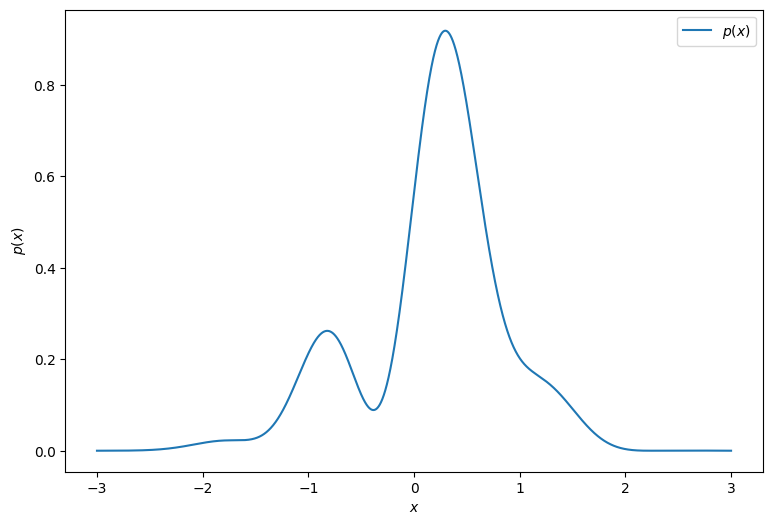
\includegraphics[width=0.7\textwidth]{./images/metropolis/example1/plot-of-px.png}
		\caption{Plot of original $p(x)$}
		\label{plot of px}
	\end{figure}

	Here, we choose,
	\[
		q(\theta_{t-1}, \theta_{t}) = q(\theta_t|\theta_{t-1}) \sim \text{N}(\theta_{t-1},\sigma^2)
	\]
	for some stander deviation $ \sigma $ that we have to select.
	Then,
	\[
		q(\theta_{t} | \theta_{t-1}) = \frac{1}{\sqrt{2 \pi \sigma^2}} \exp \left( - \frac{1}{2 \sigma^2} (\theta_t - \theta_{t-1})^2 \right)
	\]
	and,
	\[
		q(\theta_{t-1}|\theta_t) = \frac{1}{\sqrt{2 \pi \sigma^2}} \exp \left( - \frac{1}{2 \sigma^2} (\theta_{t-1} - \theta_{t})^2 \right)
	\]
	Then, it is clear that $ q(\theta_{t-1},\theta_t) = q(\theta_t.\theta_{t-1}) $

	Hence, the acceptance probability becomes,
	\begin{align*}
		\alpha(\theta_{t-1},\theta_{t}) & = \min \left(  \frac{p(\theta_t)q(\theta_t.\theta_{t-1})}{p(\theta_{t-1})q(\theta_{t-1},\theta_t)}  , 1 \right)                                                        \\
		                                & = \min \left( \frac{p(\theta_t)}{p(\theta_{t-1})} , 1 \right)                                                                                                          \\
		                                & = \min \left( \frac{e^{(-\theta_t^2)}(2 + \sin(5 \theta_t) + \sin(2 \theta_t)) }{e^{(-\theta_{t-1}^2)}(2 + \sin(5 \theta_{t-1}) + \sin(2 \theta_{t-1})) }  , 1 \right)
	\end{align*}

	Now, using various initial state and different $ \sigma $ (stander deviation of jumping distribution) simulate samples and study them.

	\textbf{Case 1:} First we choose $ 0 $ as initial state and $ \sigma = 2 $. Then after 100000 iteration we get mean of the samples to be 0.1866 and variance of the samples to be 0.4754.
	From \Cref{fig:MH sample 1 values} we can see that as we are starting from middle of our target distribution the simulated values are very good estimation of desire distribution $ p(x) $. Here we see we don't need burn-in time since from beginning the means of the sample are quite same. For the sake of tradition if we throw 25\% of samples and get 0.1900 as mean, 0.4751 as variance of the new samples and 0.3041 Geweke Z-score.

	\begin{figure}[H]
		\centering
		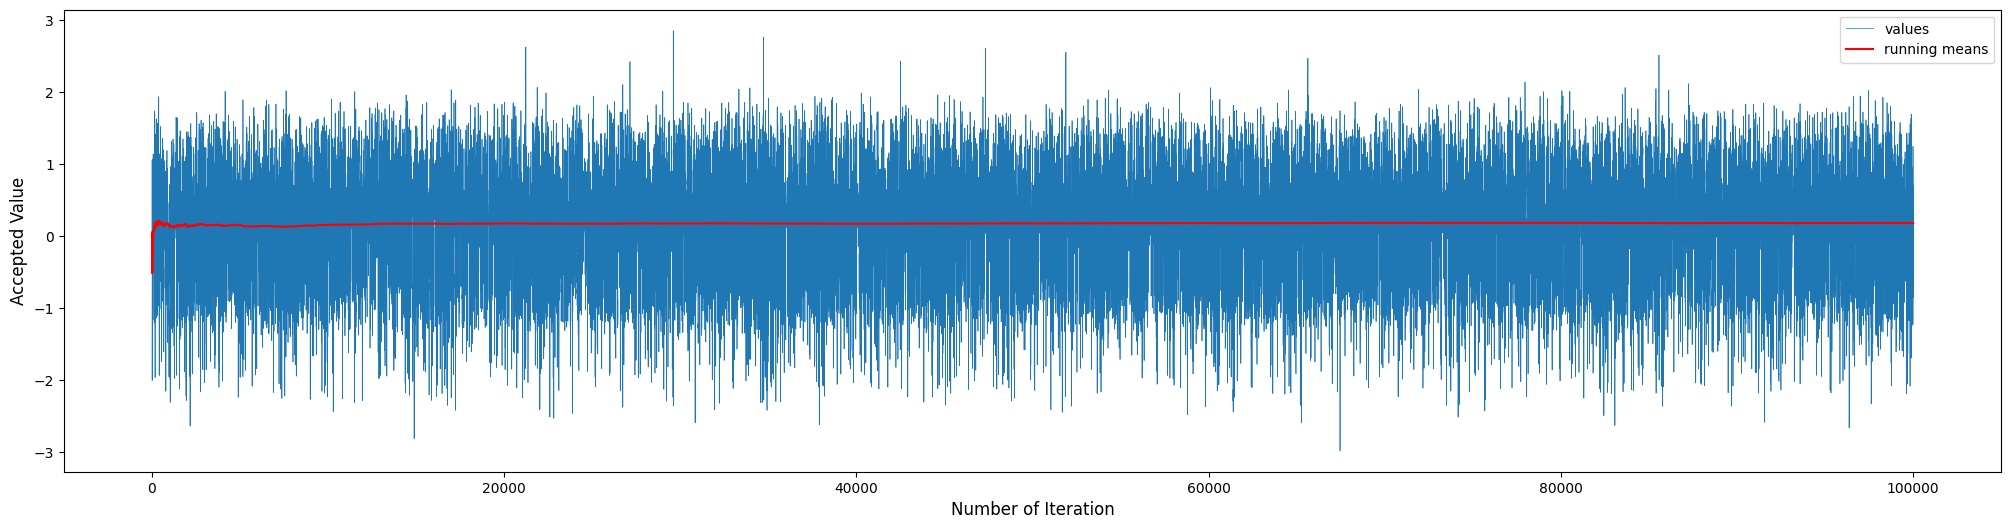
\includegraphics[width=1\textwidth]{./images/metropolis/example1/sample-1-values.png}
		\caption{Accepted values and running means for case 1 (initial state 0, $ \sigma = 2 $) before removing burn-ins}
		\label{fig:MH sample 1 values}
	\end{figure}

	\begin{figure}[H]
		\centering
		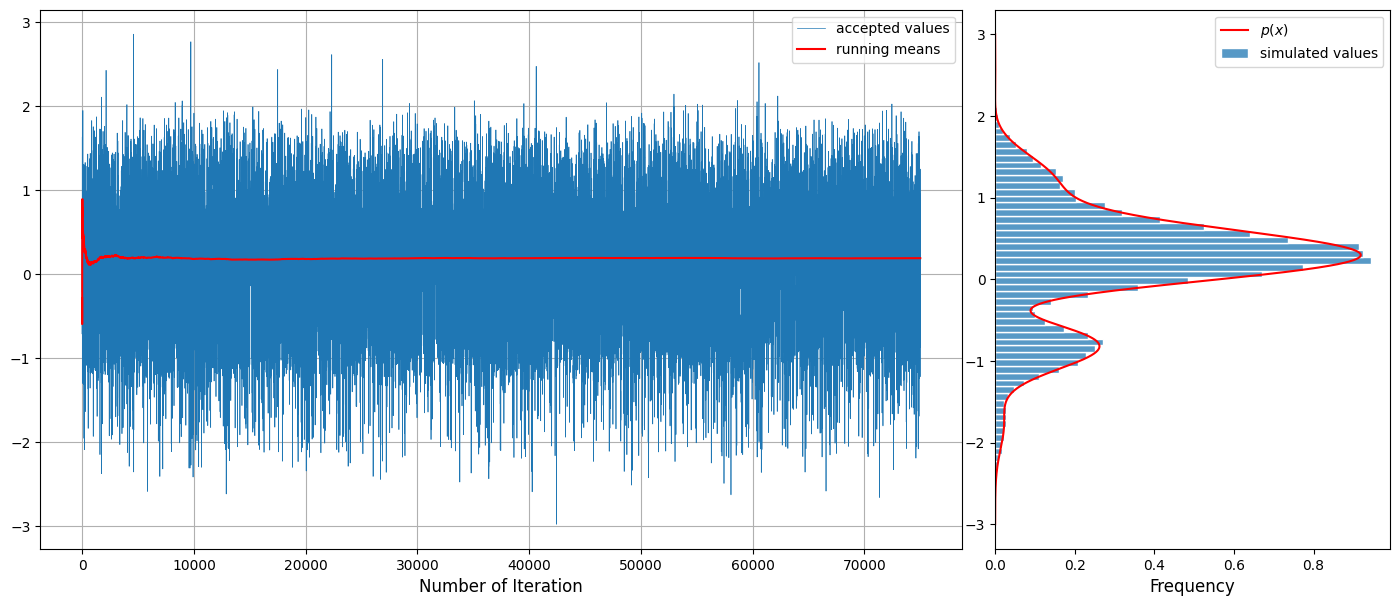
\includegraphics[width=1\textwidth]{./images/metropolis/example1/sample-1-value-hist-bo.png}
		\caption{Samples of case 1 after removing Burn-Ins}
		\label{fig:MH sample 1 after burn-in}
	\end{figure}

	\textbf{Case 2:}  Now we take -1 as initial state and $ \sigma $ to be 2, then we get mean and variance of the samples 0.1832 and 0.4641 respectively. After removing the Burn-Ins we get mean 0.17842, variance 0.47186 and Geweke Z-score 0.5433.

	\begin{figure}[H]
		\centering
		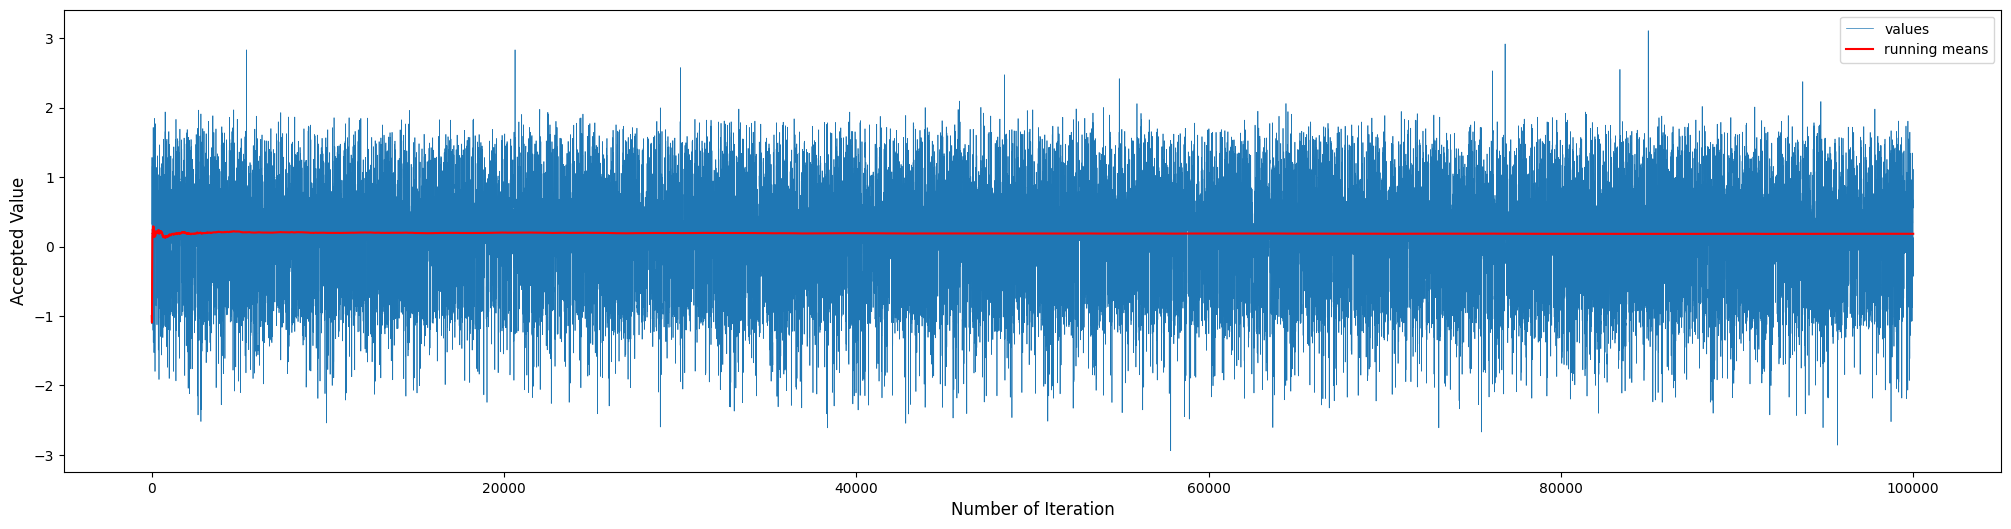
\includegraphics[width=1\textwidth]{./images/metropolis/example1/sample-2-values.png}
		\caption{Accepted values and running means for case 2 (initial state -1, $ \sigma = 2 $) before burn-in removed}
	\end{figure}

	\begin{figure}[H]
		\centering
		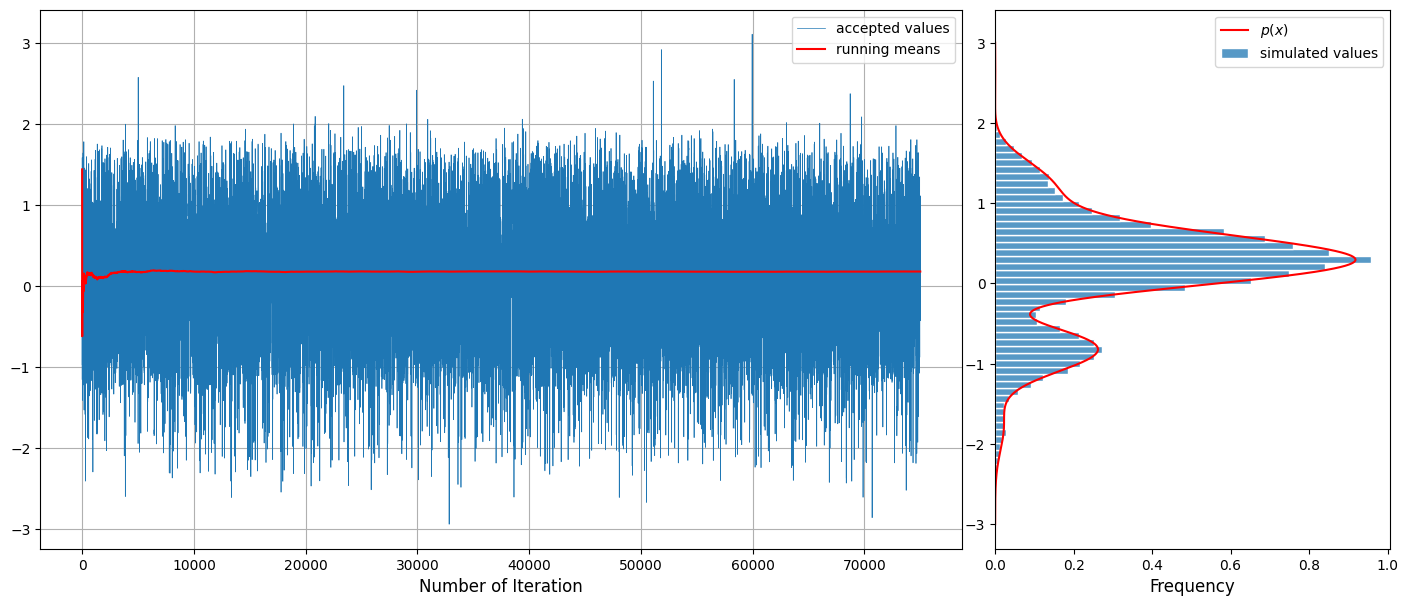
\includegraphics[width=1\textwidth]{./images/metropolis/example1/sample-2-value-hist-bo.png}
		\caption{Samples of case 2 after removing Burn-Ins}
	\end{figure}

	\textbf{Case 3:} As case 3 we take initial state to be -4 and $ \sigma = 1$, then we have mean = 0.1906, variance = 0.4686. From \Cref{fig:MH sample3} we can see for first few samples we get means to fluctuate heavily after that it is stable. So, here it is necessary to remove first few terms (Burn-In). After removing first 25\% of term we get, mean = 0.1695, variance = 0.4686 and Geweke Z-score = -0.348. Hence seeing the Geweke z-score we see after Burn-Ins are removed we get good estimation of $ p(x) $ (\Cref{fig:MH sample3 after burn in}).

	\begin{figure}[H]
		\centering
		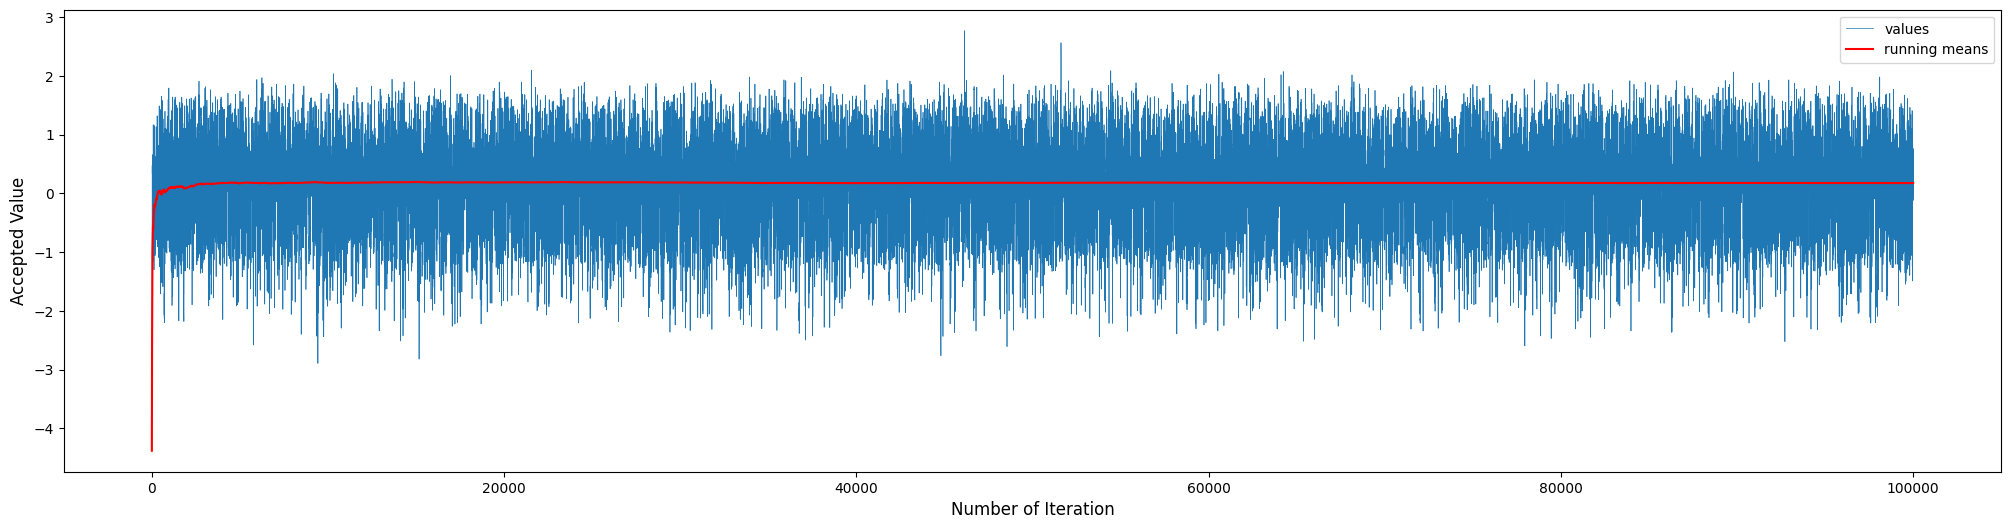
\includegraphics[width=1\textwidth]{./images/metropolis/example1/sample-3-values.png}
		\caption{Accepted values and running means for case 3 (initial state -4, $ \sigma = 1 $) before burn-in removed}
		\label{fig:MH sample3}
	\end{figure}

	\begin{figure}[H]
		\centering
		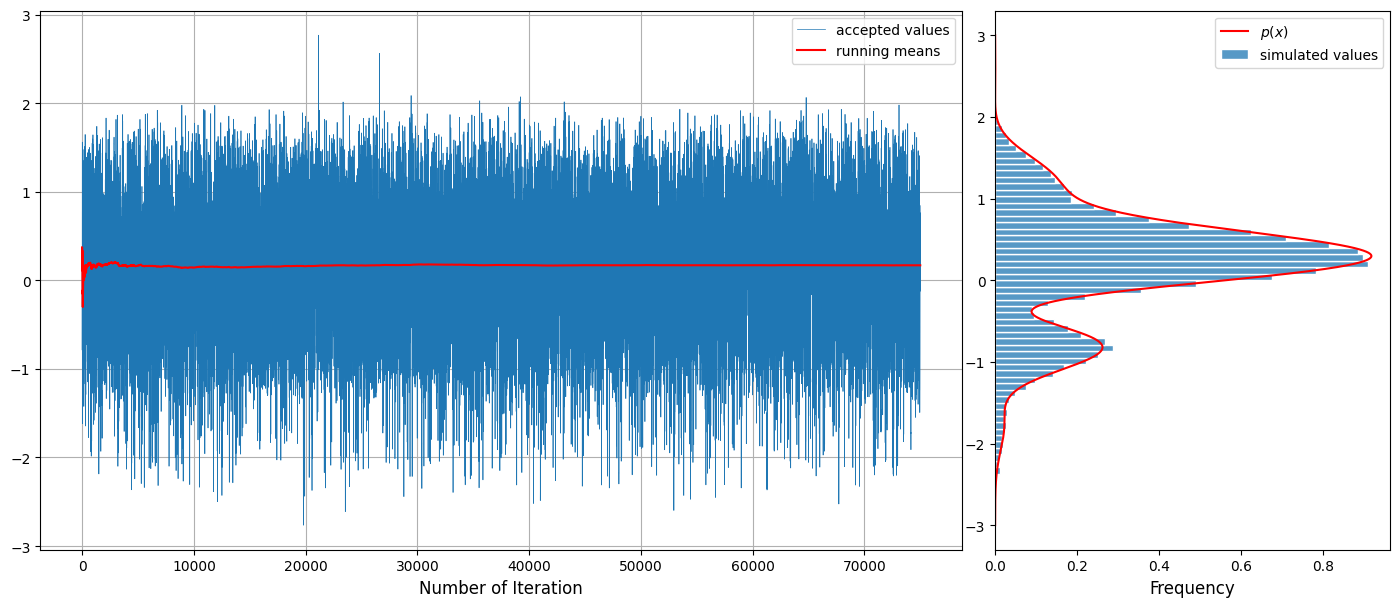
\includegraphics[width=0.9\textwidth]{./images/metropolis/example1/sample-3-value-hist-bo.png}
		\caption{Samples of case 3 after removing Burn-Ins}
		\label{fig:MH sample3 after burn in}
	\end{figure}

	\textbf{Case 4:} In this scenario, we start with an initial value far outside the desired distribution, specifically at 10, with a standard deviation of $\sigma = 2$. Observing \Cref{fig:MH sample4}, it becomes evident that removing some of the initial samples (known as Burn-Ins) is necessary. After discarding the first 25\% of the samples, we achieve a much better approximation of the target distribution. The results after this adjustment show a mean of 0.1695, a variance of 0.4686, and a Geweke Z-score of -0.4693.

	\begin{figure}[H]
		\centering
		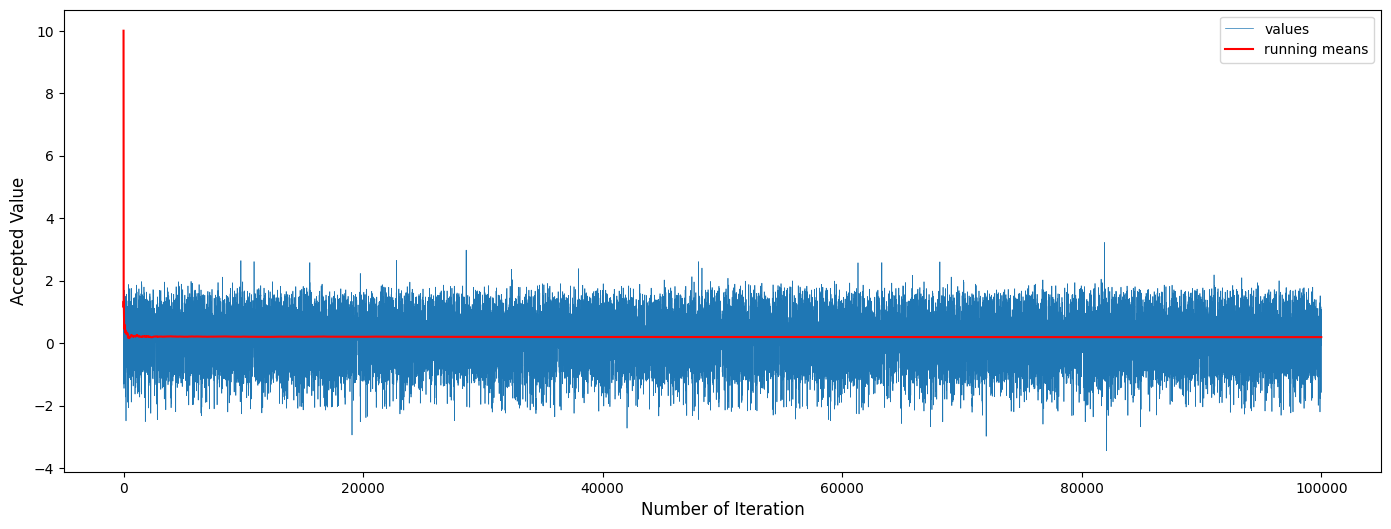
\includegraphics[width=1\textwidth]{./images/metropolis/example1/sample-4-values.png}
		\caption{Accepted values and running means for case 4 (initial state 10, $ \sigma = 2 $) before burn-in removed}
		\label{fig:MH sample4}
	\end{figure}

	\begin{figure}[H]
		\centering
		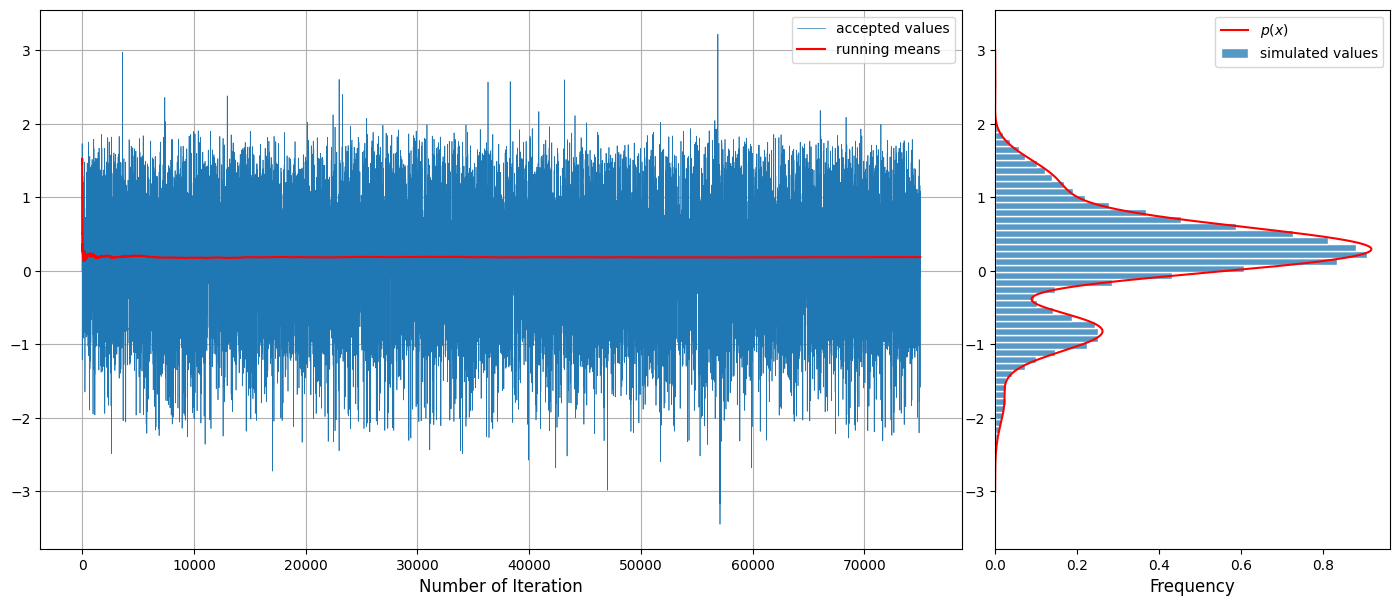
\includegraphics[width=1\textwidth]{./images/metropolis/example1/sample-4-value-hist-bo.png}
		\caption{Samples of case 4 after removing Burn-Ins}
	\end{figure}

	\textbf{Case 5:}  Now, let's examine some poor examples of the jumping distribution, using $\sigma = 0.025$ and an initial state of 10. Initially, the mean is 0.2626 and the variance of the sample is 1.4632. Although the mean is quite accurate, the high variance and triable Geweke Z-score (1.152) indicates a poor estimation, as confirmed by \Cref{fig:MH sample5}. It is crucial to remove the first 25\% of the samples. After discarding these initial samples, we obtain a mean of 0.0726 and a variance of 0.3740. With the reduced variance, this can be considered a good estimator.

	\begin{figure}[H]
		\centering
		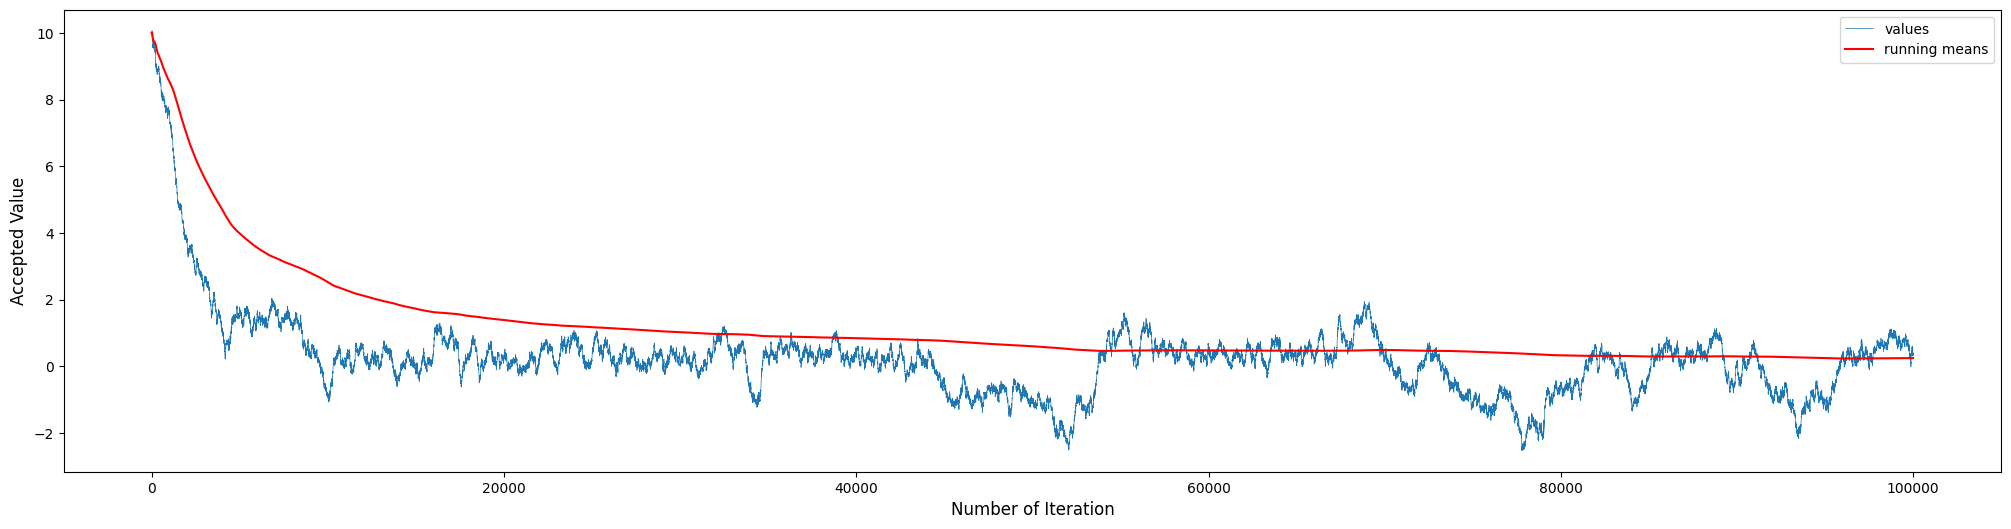
\includegraphics[width=1\textwidth]{./images/metropolis/example1/sample-5-values.png}
		\caption{Accepted values and running means for case 5 (initial state 10, $ \sigma = 0.025 $) before burn-in removed}
		\label{fig:MH sample5}
	\end{figure}

	\begin{figure}[H]
		\centering
		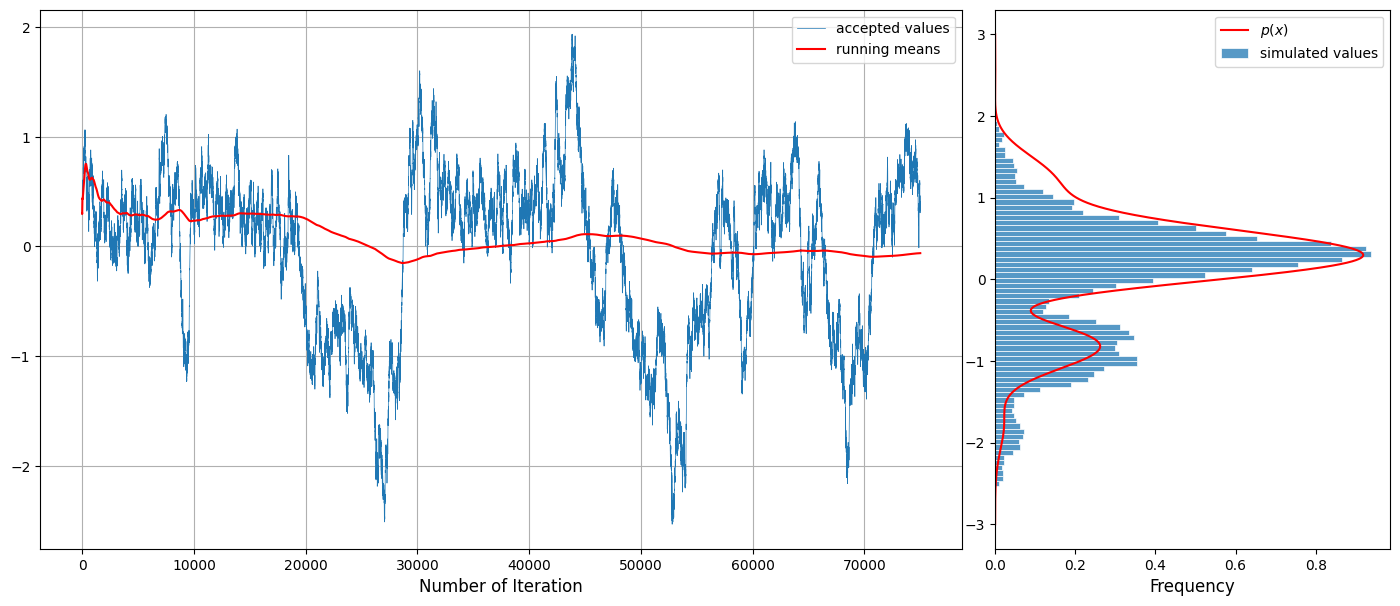
\includegraphics[width=1\textwidth]{./images/metropolis/example1/sample-5-value-hist-bo.png}
		\caption{Samples of case 5 after removing Burn-Ins}
	\end{figure}

	\textbf{Case 6:} Now we take $ \sigma $ to be 20 and initial state 15. After removing Burn-Ins we obtain mean of 0.1899, variance of 0.4423 and Geweke Z-score 3.301. Here we can see not much candidates are getting accepted and jugging from Geweke Z-score we can't accept these samples.

	\begin{figure}[H]
		\centering
		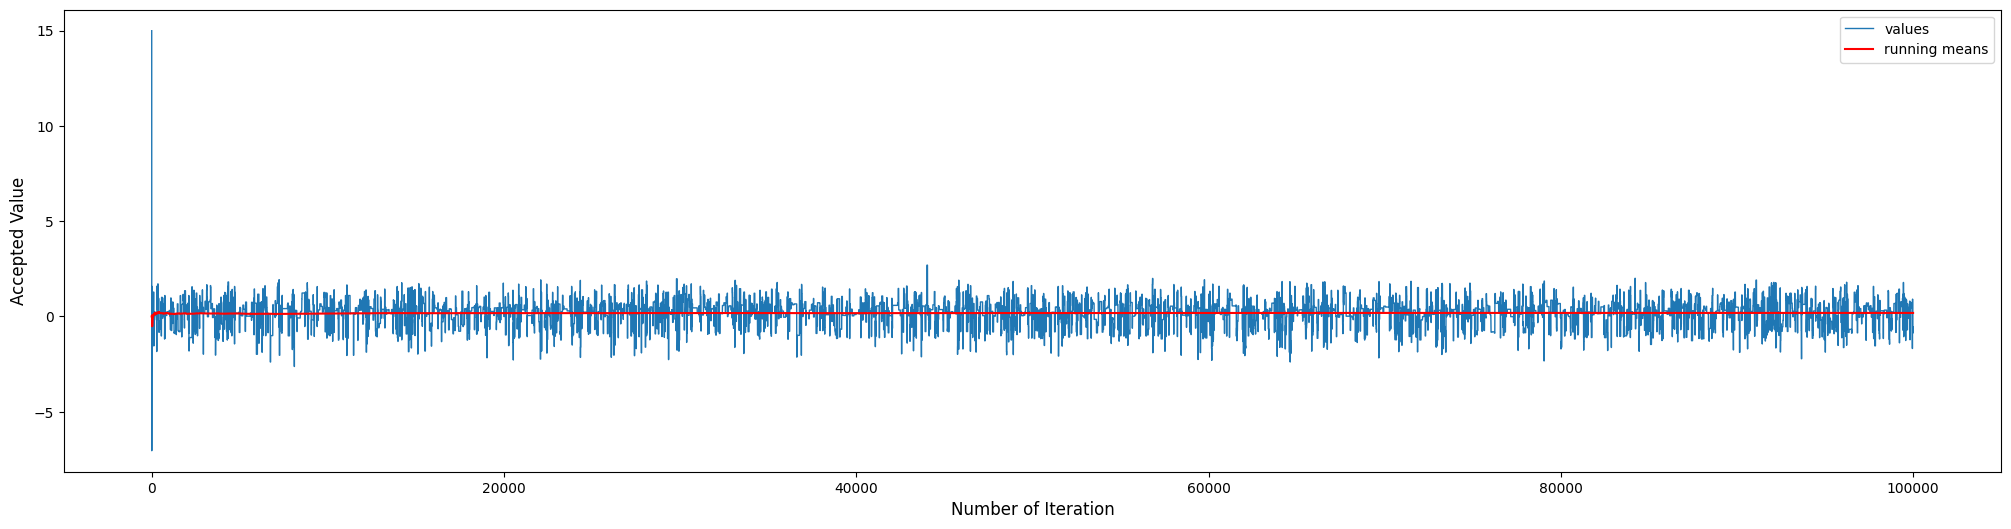
\includegraphics[width=1\textwidth]{./images/metropolis/example1/sample-6-values.png}
		\caption{Accepted values and running means for case 6 (initial state 15, $ \sigma = 20 $) before burn-in removed}
	\end{figure}

	\begin{figure}[H]
		\centering
		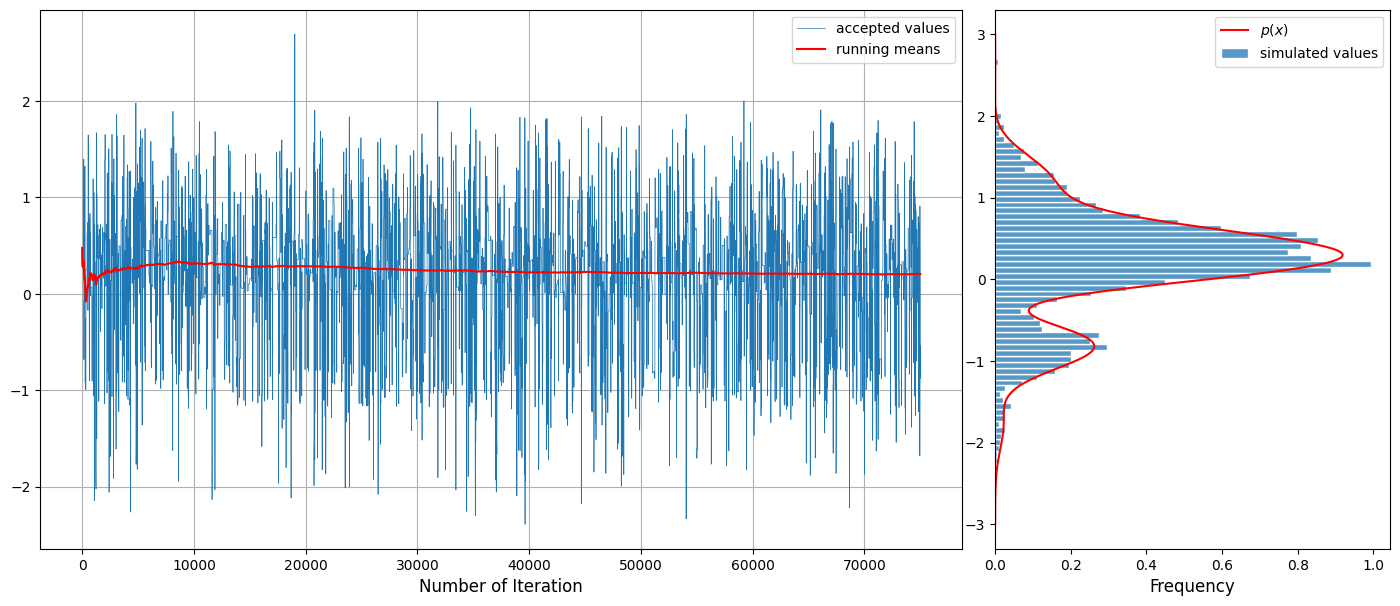
\includegraphics[width=1\textwidth]{./images/metropolis/example1/sample-6-value-hist-bo.png}
		\caption{Samples of case 6 after removing Burn-Ins}
	\end{figure}

	\begin{table}[ht]
		\centering
		\begin{tabular}{|c|p{2cm}|c|c|c|p{2cm}|p{2cm}|p{2cm}|}
			\hline
			Case & Initial State & $\sigma$ & Mean   & Variance & Mean after Burn-In & Variance after Burn-In & Geweke z-score \\ \hline
			1    & 0             & 2        & 0.1866 & 0.4754   & 0.1900             & 0.4751                 & 0.3041         \\ \hline
			2    & -1            & 2        & 0.1832 & 0.4641   & 0.17842            & 0.4718                 & 0.5433         \\ \hline
			3    & -4            & 1        & 0.1906 & 0.4686   & 0.1695             & 0.4686                 & -0.348         \\ \hline
			4    & 10            & 2        & 0.1908 & 0.4707   & 0.1695             & 0.4686                 & -0.4693        \\ \hline
			5    & 10            & 0.025    & 0.2626 & 1.4632   & 0.0726             & 0.3740                 & 1.512          \\ \hline
			6    & 15            & 20       & 0.1899 & 0.4423   & 0.1899             & 0.4423                 & 3.301          \\ \hline
		\end{tabular}
		\caption{Summary of Cases with Initial States, $\sigma$, Means, Variances, and Geweke z-test}
	\end{table}

\end{example}


\begin{example}[Finding distribution of some observed data]
	\label{eg:finding parameter}

	Another use case of Metropolis-Hastings Algorithm to find distribution of some observed data using \textbf{Bayesian Method}. Suppose we have 1000 observed samples. Now we want to find the distribution of the samples, i.e. from which distribution the samples is taken so we can generate more sample data from that distribution. Our observed data looks like \Cref{fig:observed sample}.
	\begin{figure}[H]
		\centering
		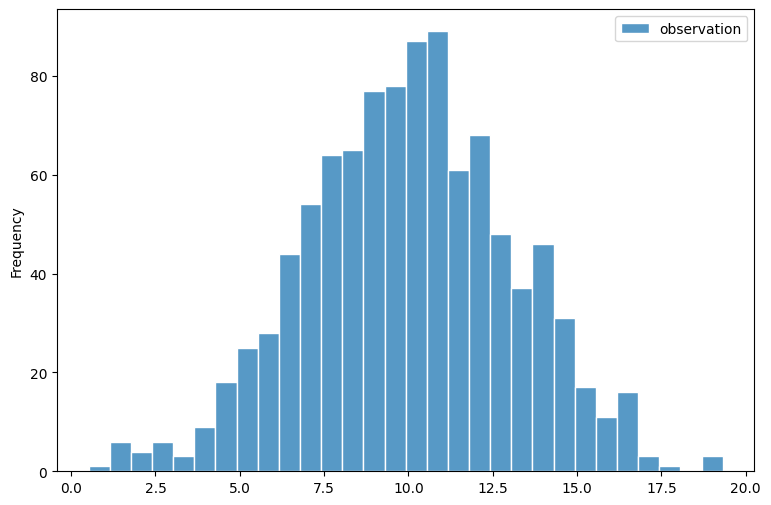
\includegraphics[width=0.6\textwidth]{images/metropolis/example2/observation.png}
		\caption{Observed Samples}
		\label{fig:observed sample}
	\end{figure}

	From \Cref{fig:observed sample} its looks like samples are form Normal Distribution with mean ($ \mu_{obs} $) 10, but we don't know the variance ($ \sigma^2 $). Using MH algorithm with the help of Bayesian method we try to find the variance. For that, at first we discuss about \textbf{Bayesian Method}.

	\begin{align*}
		P(\Theta = \theta| X=x) & = \frac{P(X=x,\Theta=\theta)}{P(X=x)}                                                                                                     \\
		                        & = \frac{P(X=x|\Theta=\theta)P(\Theta=\theta)}{\sum_{\theta}P(X=x|\Theta=\theta)P(\Theta=\theta) } \label{eq:Bayesian theorem} \numberthis
	\end{align*}

	\Cref{eq:Bayesian theorem} we know as \textbf{Bayes' theorem} for continuous case we may write \Cref{eq:Bayesian theorem} as
	\[
		f(\theta|x) = \frac{f(x|\theta)f(\theta)}{\int f(x|\theta)f(\theta)d \theta } \label{eq:Bayes theorem for continuous} \numberthis
	\]
	here, the probability density $ f(\theta) $ is called \textbf{prior distribution}, $ f(\theta|x) $ is known as \textbf{posterior distribution}

	If we have $ n $ IID observations $ X_1,X_2,X_3,\ldots,X_n $, we replace $ f(x|\theta) $ with
	\[
		f(x_1,x_2,\ldots,x_n|\theta) = \prod_{i=1}^{n} f(x_i|\theta) = \mathcal{L}_n(\theta)
	\]
	$ \mathcal{L}_n(\theta) $ is known as \textbf{likelihood function}. Now, we denote $ X^{n} = (X_1,X_2,\ldots,X_n) $ and $ x_n = (x_1,x_2,\ldots,x_n) $.

	Now,

	\begin{equation}
		f(\theta|x^{n} ) = \frac{f(x^{n}|\theta)f(\theta) }{\int f(x^{n}|\theta)f(\theta)d \theta } = \frac{\mathcal{L}_n(\theta)f(\theta)}{\int \mathcal{L}_n(\theta) f(\theta)d \theta} \propto \mathcal{L}_n(\theta)f(\theta)
	\end{equation}

	Since, $ \int \mathcal{L}_n(\theta)f(\theta)d \theta  $ does not depend on $ \theta $

	So, we can summarize Bayesian Method to be
	\[
		f(\theta|x^{n} ) \propto \mathcal{L}_n(\theta)f(\theta) \label{eq:bayesian method} \numberthis
	\]
	choosing some prior beliefs using some observed data we upgrade our beliefs and calculate the posterior.

	Now coming to our example write the \Cref{eq:bayesian method} as,

	\[
		f(\sigma|D,\theta) \propto \mathcal{L}_n(\sigma)f(\sigma)
	\]

	Here, we are taking the prior to be $ f(\sigma) $ as $ \mu $ is constant and
	\[
		f(d_i|\mu,\sigma) = \frac{1}{\sqrt{2 \pi \sigma^2}} \exp \left( - \frac{(d_i -\mu )^2}{2 \sigma^2} \right)
	\]
	then, likelihood function is given by,
	\[
		\mathcal{L}_n(\sigma) = \prod_{i=1}^{n} f(d_i|\mu,\sigma) = \prod_{i=1}^{n} \left( \frac{1}{\sqrt{2 \pi \sigma^2}} \exp \left( - \frac{(d_i -\mu )^2}{2 \sigma^2} \right) \right)
	\]

	Now the question is that how we choose prior? If we know $ \sigma $ can't be negative as $ \sigma = \sqrt{ \frac{1}{n} \sum_{i}^{n} (d_i - \mu)^2 } $. So we take,

	\[
		f(\sigma) =
		\begin{cases}
			0, \ \ \sigma \le 0 \\
			1, \ \ \sigma > 0
		\end{cases} \numberthis \label{eq:prior}
	\]

	We take \textbf{jumping distribution}  to be,
	\[
		q(\sigma_{t+1}|\sigma_{t}) = \text{N}(\sigma_t,1) \label{eq:jumping for mh example2} \numberthis
	\]
	Now, for acceptance probability,
	we accept $ \sigma_{t+1} $ if,
	\begin{equation}
		\label{eq:1st accept mh example2}
		\frac{\mathcal{L}_n(\sigma_{t+1})f(\sigma_{t+1})}{\mathcal{L}_n(\sigma_{t})f(\sigma_{t})} \ge 1
	\end{equation}
	If the ratio is less than 1, then we compare it to a uniform random number from $ [0,1] $. If the ratio is larger or equal to the random number we accept $ \sigma_{t+1} $ else we reject it.

	Now we take $ \log $ on the both side of \Cref{eq:1st accept mh example2}. Since $ \log $ is increasing function, so sign will be same then we have,
	\begin{gather*}
		\log \left(  \mathcal{L}_n(\sigma_{t+1})f(\sigma_{t+1}) \right) - \log \left(  \mathcal{L}_n(\sigma_{t})f(\sigma_{t})\right) \ge 0 \\
		\text{or, } \log( \mathcal{L}_n(\sigma_{t+1}) ) + \log(f(\sigma_{t+1})) \ge \log(\mathcal{L}_n(\sigma_t)) + \log(f(\sigma_t)) \\
		\text{or, } \sum_{i=1}^n \log(f(d_i|\mu,\sigma_{t+1})) + \log(f(\sigma_{t+1}))  \ge \sum_{i = 1}^{n} \log(f(d_i|\mu,\sigma_t)) + \log (f(\sigma_t))\\
		\text{or, } \sum_{i = 1}^{n} \left( \log(\sigma_{t+1}\sqrt{2 \pi}) - \left( \frac{(d_i - \mu)^2}{2 \sigma_{t+1}^2} \right) \right) + \log(f(\sigma_{t+1})) \ge \\ \sum_{i = 1}^{n} \left( \log(\sigma_{t}\sqrt{2 \pi}) - \left( \frac{(d_i - \mu)^2}{2 \sigma_{t}^2} \right) \right) + \log(f(\sigma_{t})) \label{eq:2nd accept mh example2} \numberthis
	\end{gather*} \\
	Now, we accept $ \sigma_{t+1} $ if it satisfies \Cref{eq:2nd accept mh example2} or if not satisfies the Equation we calculate $ \alpha(\sigma_{t+1},\sigma_t) $ by,

	\begin{align*}
		\alpha(\sigma_{t+1}, \sigma_t) = \exp \bigg( & \sum_{i=1}^{n} \left( \log(\sigma_{t+1} \sqrt{2 \pi}) - \frac{(d_i - \mu)^2}{2 \sigma_{t+1}^2} \right) + \log(f(\sigma_{t+1})) \\
		                                             & - \sum_{i=1}^{n} \left( \log(\sigma_t \sqrt{2 \pi}) - \frac{(d_i - \mu)^2}{2 \sigma_t^2} \right) + \log(f(\sigma_t)) \bigg)
	\end{align*}
	and accept $ \sigma_{t+1} $ with probability $ \alpha $

	But why take $ \log $? Because, it helps with analytical precision, i.e. multiplying thousand of small values may case an underflow in the system's memory (situation where a number is so close to zero that it cannot be represented accurately within the given precision of the system's floating point representation.). $ \log $ is perfect solution because it transforms multiplication to additions and small positive numbers into non-small negative numbers.

	Now, using \Cref{eq:prior} as \textbf{prior}, \Cref{eq:jumping for mh example2} as \textbf{jumping distribution}, \Cref{eq:2nd accept mh example2} as acceptance scam and $0.1$ to be initial state we use Metropolis-Hastings Algorithm.

	\begin{figure}[H]
		\centering
		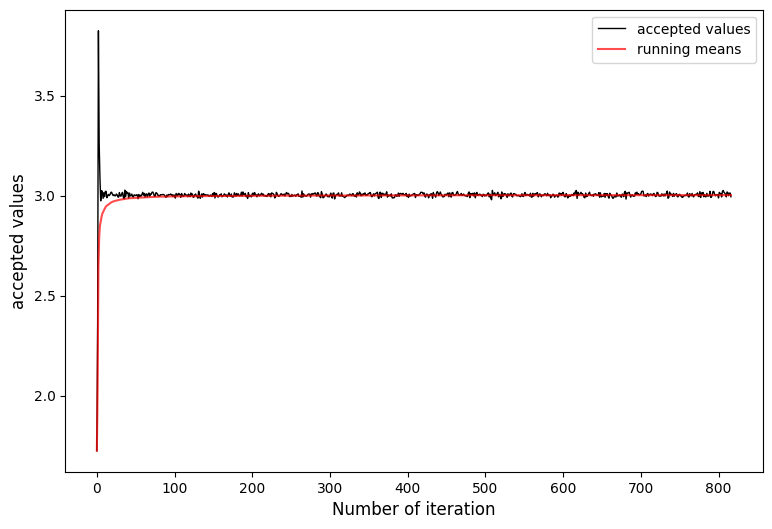
\includegraphics[width=0.7\textwidth]{images/metropolis/example2/values.png}
		\caption{Accepted values from Metropolis-Hastings Algorithm}
		\label{fig:example2 values}
	\end{figure}

	After running 100000 iteration we only accepted 817 values and values are looks like \Cref{fig:example2 values}. Here we can see we have to throw Burn-Ins (first 25\% sample). After removing Burn-Ins we get our desire samples to estimate $ \sigma $.

	\begin{figure}[H]
		\centering
		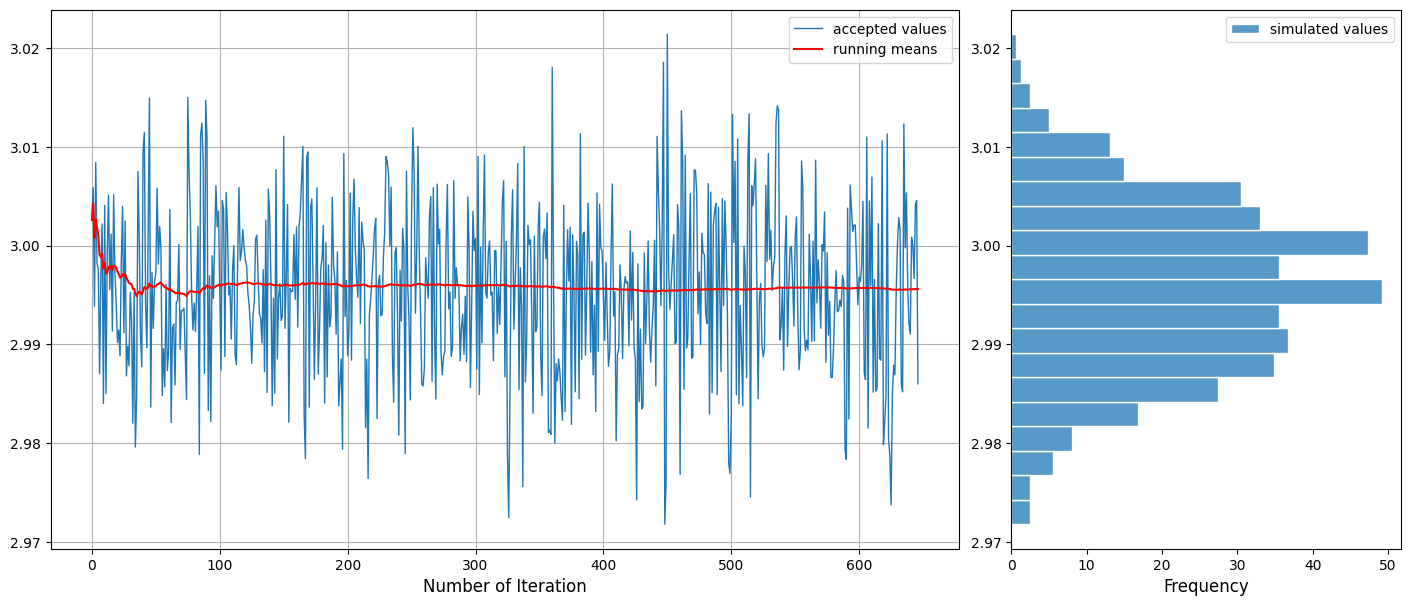
\includegraphics[width=1\textwidth]{images/metropolis/example2/values-after-burnin.png}
		\caption{Accepted values after removing Burn-Ins}
	\end{figure}

	From this we get our desire values of $ \sigma $ to be 3.0032, variance of the samples to be 0.0001 and 0.05545 as Geweke Z-score. Because of low variance and Geweke Z-score less than 2 for simulated data we conform that it is very good estimate.

	As a matter of fact I have taken observed values from $ \text{N}(10,9) $ distribution. So, we see the algorithm is very accurate to finding the means.

	\begin{figure}[H]
		\centering
		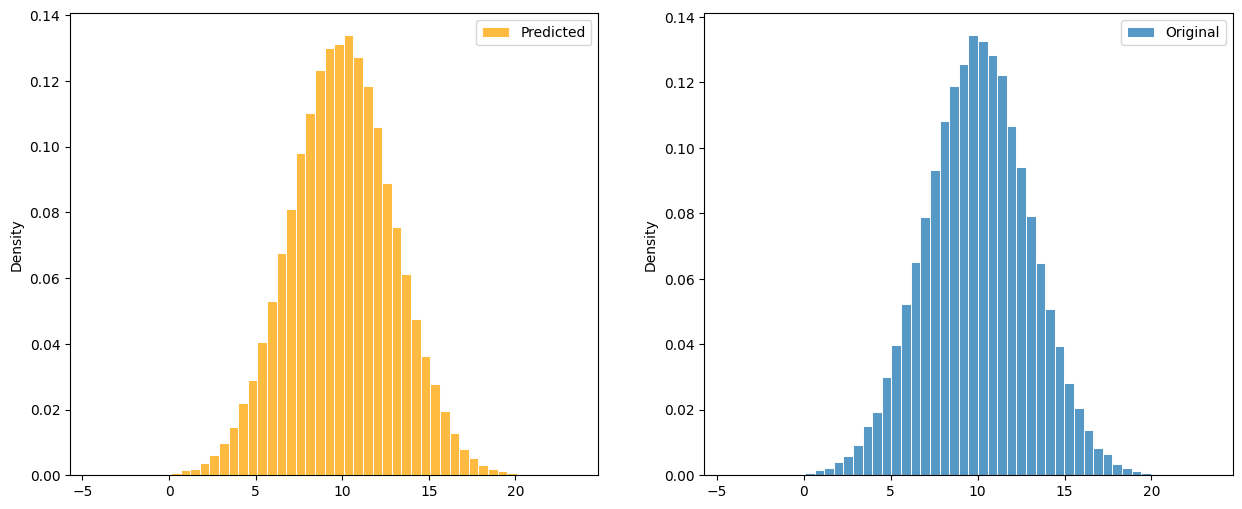
\includegraphics[width=1\textwidth]{images/metropolis/example2/original-with-simulated.png}
		\caption{Original population with simulated samples}
	\end{figure}

\end{example}







